\documentclass[10pt,a4paper]{article}
\usepackage[T1]{fontenc}
\usepackage{mathpazo}
\usepackage{microtype}
\usepackage{amsmath,amssymb}
\usepackage{graphicx}
\usepackage{booktabs}
\usepackage{xcolor}
\usepackage{fancyhdr}
\usepackage{titlesec}
\usepackage{tikz}
\usepackage[font=small,labelfont=bf,labelsep=colon,skip=3pt]{caption}
\usepackage{subcaption}
\usepackage{enumitem}
\usepackage{tocloft}
\usepackage{float}
\usepackage{fancyvrb}
\usepackage[a4paper,left=1.8cm,right=1.8cm,top=1.9cm,bottom=1.7cm,headheight=14pt]{geometry}
\usepackage[colorlinks=true,linkcolor=ramen,urlcolor=ramen,citecolor=ramen]{hyperref}
\usetikzlibrary{arrows.meta,positioning,shapes.geometric,calc,fit,backgrounds}

\definecolor{ramen}{HTML}{8B2A1A}
\definecolor{ramenlt}{HTML}{F6E9E2}
\definecolor{ink}{HTML}{333333}
\definecolor{okgreen}{HTML}{2E7D32}
\graphicspath{{figs/}}

\setlength{\parindent}{0pt}
\setlength{\parskip}{3pt}
\renewcommand{\arraystretch}{1.1}
\titleformat{\section}{\Large\bfseries\color{ramen}}{\thesection}{0.6em}{}
\titleformat{\subsection}{\large\bfseries\color{ink}}{\thesubsection}{0.5em}{}
\titlespacing*{\section}{0pt}{8pt}{3pt}
\titlespacing*{\subsection}{0pt}{6pt}{2pt}
\setlist[itemize]{noitemsep,topsep=2pt,leftmargin=1.3em}
\setlist[enumerate]{noitemsep,topsep=2pt,leftmargin=1.5em}
\captionsetup[figure]{aboveskip=3pt,belowskip=0pt}
\captionsetup[subfigure]{font=footnotesize,labelfont=bf,skip=1pt}
\setlength{\textfloatsep}{7pt plus 2pt minus 2pt}
\setlength{\floatsep}{5pt plus 2pt minus 2pt}
\setlength{\intextsep}{5pt plus 2pt minus 2pt}
\fvset{fontsize=\scriptsize,frame=lines,framesep=1.5mm,rulecolor=\color{ramen!50}}

\pagestyle{fancy}
\fancyhf{}
\fancyhead[L]{\small\color{gray}3D Ramen Shop: A Japanese Ramen Restaurant in OpenGL}
\fancyhead[R]{\small\color{gray}CSE 4102}
\fancyfoot[C]{\small\thepage}
\renewcommand{\headrulewidth}{0.4pt}

\renewcommand{\cftsecfont}{\bfseries\footnotesize}
\renewcommand{\cftsecpagefont}{\bfseries\footnotesize}
\renewcommand{\cftsubsecfont}{\scriptsize}
\renewcommand{\cftsubsecpagefont}{\scriptsize}
\setlength{\cftbeforesecskip}{2pt}
\setlength{\cftbeforesubsecskip}{0pt}
\renewcommand{\cfttoctitlefont}{\Large\bfseries\color{ramen}}
\setlength{\cftaftertoctitleskip}{3pt}

\tikzset{
  box/.style={draw=ramen!70,fill=ramenlt,rounded corners=2pt,align=center,font=\scriptsize,inner sep=3pt,minimum height=0.55cm},
  arr/.style={-{Stealth[length=4pt]},draw=ramen!80!black,thick},
  lab/.style={font=\tiny,inner sep=1pt}
}
\newcommand{\code}[1]{\texttt{\small #1}}
\newcommand{\fig}[2]{\includegraphics[width=#1\linewidth]{#2}}
\newcommand{\yes}{\textcolor{okgreen}{\textbf{Implemented}}}
\newcommand{\no}{\textcolor{red!70!black}{\textbf{Not implemented}}}
\newcommand{\adapt}{\textcolor{orange!80!black}{\textbf{Adapted}}}

\begin{document}

% ===================== COVER =====================
\thispagestyle{empty}
\begin{center}
{\large\bfseries Khulna University of Engineering \& Technology (KUET)}\\[1pt]
Department of Computer Science and Engineering\\[4pt]
{\small\color{gray} CSE 4102 \,$\cdot$\, Computer Graphics and Image Processing Laboratory \,$\cdot$\, 4th Year, 1st Term}\\[8pt]
{\fontsize{30}{36}\selectfont\bfseries\color{ramen} The Ramen Shop}\\[2pt]
{\large Project Report: A Japanese Ramen Village in OpenGL}\\[6pt]
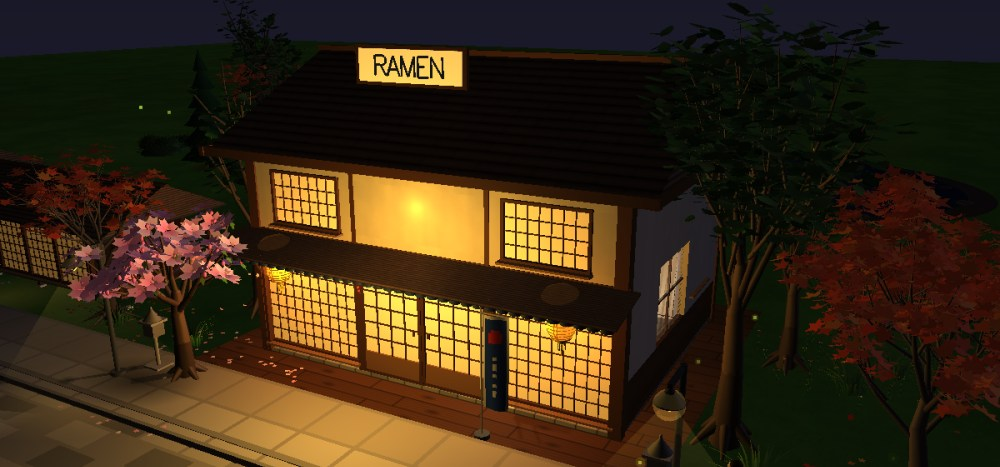
\includegraphics[width=0.74\textwidth]{fig_ext_night.jpg}\\[1pt]
{\small\color{gray} The shop at night, rendered in real time by the project.}
\end{center}
\vspace{4pt}
\begin{minipage}[t]{0.46\textwidth}
{\bfseries\color{ramen} Submitted by}\\[1pt]
\textbf{Rajorshi Das}\\ Roll: 2107060\\ Dept.\ of CSE, KUET
\end{minipage}\hfill
\begin{minipage}[t]{0.50\textwidth}
{\bfseries\color{ramen} Submitted to}\\[1pt]
\textbf{Md Tajmilur Rahman}, Lecturer, Dept.\ of CSE, KUET\\
\textbf{Md. Mubtashim Abrar Nihal}, Lecturer, Dept.\ of CSE, KUET
\end{minipage}
\vspace{4pt}
\begin{center}
{\small\color{gray} C++17 \,$\cdot$\, OpenGL (fixed function + GLSL 1.20) \,$\cdot$\, FreeGLUT \,$\cdot$\, GLEW \,$\cdot$\, October 2026}
\end{center}
\vspace{2pt}
{\small\setcounter{tocdepth}{1}\tableofcontents}
\newpage

% ===================== 1 INTRODUCTION =====================
\section{Introduction}
\textbf{The Ramen Shop} is an interactive 3D Japanese village written from scratch in C++ and OpenGL. A two-storey ramen shop (dining counter, open kitchen, two tables, an upstairs tatami room) stands on a cobblestone street with ten neighbouring houses, street lamps, many trees, a lawn and a lake with ducks. The sky has a sun, moon, stars and clouds and changes between day and night; a cyclist, a walking person and a cat move in the street, and a small ramen-cooking game can be played in the shop. All objects are built from basic shapes and all textures are generated by the program, so no model or image file is used.

This report explains \emph{what was proposed, what was implemented, how each feature was implemented, and which theory, formula or equation it uses}, so that the implementation can be explained from the report alone. Screenshots from the running program are given as results of each feature.

\textbf{Objectives.} (1)~Model a believable multi-part scene from basic shapes using 3D transformations. (2)~Light it with the ambient, diffuse and specular terms, with several lights that can be switched. (3)~Apply procedurally generated textures, and shade with Gouraud and Phong shading. (4)~Add shadows, glass refraction and ray tracing. (5)~Make the scene alive and explorable: animation, several cameras, mouse and keyboard interaction, and a small game.

% ===================== 2 PROPOSAL vs IMPLEMENTATION =====================
\section{Proposed Features and What Was Implemented}
Table~\ref{tab:map} compares the features of the proposal with the final project, and gives the section where each is explained.
\begin{table}[htbp]
\centering\small
\begin{tabular}{@{}p{3.6cm}p{2.6cm}p{8.3cm}c@{}}
\toprule
\textbf{Proposed feature} & \textbf{Status} & \textbf{How it appears in the final project} & \textbf{Sec.}\\
\midrule
Translation & \yes & cyclist, person, cat, ducks, sliding doors, steam, falling petals & \ref{sec:xf}\\
Rotation & \yes & wheels, cranks, fan blades, hinged door, chime pendulums, pivot sway of trees & \ref{sec:xf}\\
Scaling & \yes & boards from cubes, ellipsoids, cat $\times1.8$, user scaling of objects (keys \code{,} \code{.}) & \ref{sec:xf}\\
Perspective camera & \yes & 45$^\circ$ (62$^\circ$ in game); seven cameras & \ref{sec:view}\\
Orthographic view & \adapt & used for the game HUD, order board and title screen, not for inspecting the scene & \ref{sec:view}\\
Hierarchical modelling & \yes & cyclist, person, cat, wind chime, trees, lanterns & \ref{sec:xf}\\
Lighting: ambient, diffuse, specular & \yes & 8 lights (directional, point, spot), each term switchable & \ref{sec:light}\\
Flat shading & \no & only smooth shading is used (Gouraud or Phong) & \ref{sec:shade}\\
Gouraud shading & \yes & fixed-function path, key \code{G} & \ref{sec:shade}\\
Phong shading & \yes & own GLSL fragment shader, per-pixel, 8 lights & \ref{sec:shade}\\
Skybox & \yes & gradient dome, sun, moon, stars, clouds, day / night & \ref{sec:sky}\\
Textures & \yes & 13 procedural textures (grass, wood, tile, tatami, \ldots), mipmaps & \ref{sec:tex}\\
\midrule
\multicolumn{4}{@{}l}{\textbf{Features added beyond the proposal}}\\
\midrule
Shadows & \yes & stencil projected shadows, soft shadow map with PCF & \ref{sec:shadow}\\
Glass refraction & \yes & screen-space refraction of the tumbler & \ref{sec:glass}\\
Ray tracing & \yes & CPU ray tracer with BVH: reflection, refraction (pots, bowls, ball, mirror) & \ref{sec:rt}\\
Animated characters & \yes & cyclist with inverse kinematics, walking person, cat state machine & \ref{sec:anim}\\
Environment & \yes & trees by recursion, flowers, lake, ducks, 10 houses, street, fireflies & \ref{sec:env}\\
Cooking game & \yes & state machine, scoring, HUD & \ref{sec:game}\\
\bottomrule
\end{tabular}
\caption{Proposed features and their final status.}\label{tab:map}
\end{table}

% ===================== 3 TOOLS AND SOURCES =====================
\section{Tools, Libraries and Sources Followed}
\begin{table}[htbp]
\centering\small
\begin{tabular}{@{}p{3.0cm}p{13.3cm}@{}}
\toprule
Language, build & C++17, Visual Studio (MSBuild), x64 Release / Debug; about 15\,000 lines in 18 source files and 17 headers\\
Graphics API & OpenGL fixed-function pipeline plus GLSL 1.20 shaders (Phong lighting, glass refraction, ray-trace compositing); framebuffer objects and float textures (OpenGL 3.0)\\
Libraries & FreeGLUT (window, input), GLEW (extensions), GLU (quadrics, \code{gluLookAt}, \code{gluPerspective}, \code{gluUnProject}); NuGet package \code{nupengl.core}\\
Assets & none: no model, texture, image or sound file is loaded; all geometry is generated in code and all textures are painted by the program at start-up\\
\bottomrule
\end{tabular}
\caption{Tools and libraries.}
\end{table}
\textbf{Sources and references followed.} The algorithms follow the standard references: the Phong reflection model~[1], Blinn's half-vector specular term~[2], Gouraud interpolation~[3], Whitted's recursive ray tracing~[4], Williams' shadow maps and percentage-closer filtering~[5,6], Schlick's Fresnel approximation~[7], the Sutherland--Hodgman polygon clipping algorithm~[8] and the OpenGL specification and programming guide~[9]. Value noise and fractal Brownian motion for the textures follow the usual procedural-texture technique~[10]. The Beach Day project report was used only as a guide to the layout of a report. Library functions are used as documented; the scene, the shaders, the textures, the ray tracer and the animation code are implemented in the project itself.

% ===================== 4 ARCHITECTURE =====================
\section{Program Structure}
One world coordinate system: $x$ right, $y$ up, $z$ toward the street, one unit about one metre. The ground floor is $9.8\times7.8$ and $3.3$ high, the upper floor $2.0$, the lawn 240 units wide, the road and sidewalks at $z\approx7$--$17$, and the lake behind the shop at $(0,-24)$.
\begin{table}[htbp]
\centering\small
\begin{tabular}{@{}p{4.3cm}p{12.0cm}@{}}
\toprule
\textbf{Files} & \textbf{Responsibility}\\
\midrule
\code{main}, \code{camera} & window, frame loop, 16\,ms timer, seven cameras, keyboard and mouse\\
\code{shapes}, \code{texture} & primitives and materials; all 13 procedural textures\\
\code{scene}, \code{exterior} & sky, ground, shop, upstairs room, cyclist, person, cat, chime, houses, trees, lake, props\\
\code{furniture}, \code{food}, \code{decorations} & counter, kitchen, tables, bowls and food, lanterns, noren, clock\\
\code{lighting}, \code{shader} & the 8 lights, day / night, Phong shader, fog\\
\code{shadowmap}, \code{refraction} & soft shadow mapping, screen-space glass\\
\code{rtcore}, \code{rtscene}, \code{rtpass} & ray tracer, the shop as the rays see it, threaded pass and compositing\\
\code{objects}, \code{game} & selectable / movable objects, the ramen game\\
\bottomrule
\end{tabular}
\caption{Modules of the program.}
\end{table}
At start-up the program opens the window (double buffer, depth, stencil), paints the 13 textures and builds mipmaps, sets up the lights and fog, compiles the shaders and creates the shadow-map and glass framebuffers. Every frame it (1)~reads input and advances the animation clock \code{animTime}; (2)~sets the camera and the 45$^\circ$ projection and updates light positions and colours; (3)~renders the shadow map; (4)~draws the sky, lawn and street, the sun shadows, the exterior and then the interior; (5)~applies glass refraction, then the ray-tracing pass; (6)~draws the HUD with an orthographic projection and swaps buffers.

% ===================== 5 IMPLEMENTATION =====================
\section{Implementation of Each Feature}

\subsection{3D modelling from basic shapes}\label{sec:model}
\textbf{Theory.} Complex objects are unions of simple solids. A cylinder/cone with radii $r_0,r_1$ and height $h$ is a frustum; a \emph{surface of revolution} (lathe) turns a profile $(r(s),y(s))$ about the $y$ axis:
\begin{equation}
\mathbf p(s,\theta)=\big(r(s)\cos\theta,\ y(s),\ r(s)\sin\theta\big),\qquad \mathbf n\propto\big(y'\cos\theta,\ -r',\ y'\sin\theta\big).
\end{equation}
A grid surface samples a height function $z=f(u,v,t)$ on a mesh of quads; a tree is a recursive (self-similar) structure.\\
\textbf{Implementation.} \code{shapes.cpp} provides \code{drawCube}, \code{drawCuboid}, \code{drawCylinder}, \code{drawCone}, \code{drawSphere}, \code{drawTorus}, \code{drawPlane}, \code{drawWedge} and textured boxes. Bowls, lamp shades, bottles and the wind-chime bell are lathes; the nobori banner is a $12\times28$ grid with $z(u,v,t)=(0.09\sin(3.2t-4u+1.5v)+0.015\sin(5.1t+3v))\,u$ and the normal from $\partial z/\partial u$. A tree is built by \code{growBranch}:
\begin{Verbatim}
growBranch(base, dir, len, r, level):
    p1 = base + 0.55*len*dir;  p2 = p1 + 0.45*len*dir2        // two tapered tubes
    tube(base,p1,r,0.72r);  tube(p1,p2,0.72r,0.48r)
    if level < maxLevel:
        for k in 1..(level==1 ? 3 : 2):                       // children at random angle
            theta = 0.45+0.45*rnd();  phi = 2*pi*rnd()
            growBranch(start_k, rotate(dir,theta,phi), 0.6*len, 0.55r, level+1)
        growBranch(p2, dir2, 0.55*len, 0.45r, level+1)        // the branch continues
    leafOrBlossomCluster(p2)                                  // leaves at the tips
\end{Verbatim}
The result is compiled into OpenGL display lists once (trunk plus seven swaying branch groups, three variants plus a lighter distance version).

\subsection{Transformations and hierarchical modelling}\label{sec:xf}
\textbf{Theory.} Points are homogeneous 4-vectors, so translation, scaling and rotation are matrices:
\begin{equation}
T(\mathbf p)=\begin{pmatrix}1&0&0&p_x\\0&1&0&p_y\\0&0&1&p_z\\0&0&0&1\end{pmatrix},\
S=\mathrm{diag}(s_x,s_y,s_z,1),\
R_z(\theta)=\begin{pmatrix}\cos\theta&-\sin\theta&0&0\\\sin\theta&\cos\theta&0&0\\0&0&1&0\\0&0&0&1\end{pmatrix}.
\end{equation}
They compose by multiplication, applied right to left, so $M=T\,R\,S$ scales first and moves last. Rotation about a pivot $\mathbf c$ is $T(\mathbf c)R(\theta)T(-\mathbf c)$. A matrix stack (\code{glPushMatrix}/\code{glPopMatrix}) lets a child part be drawn in the frame of its parent.\\
\textbf{Implementation.} Every object is placed by one function, \code{applyTransform(pos, rot, scale)} $=T\,R_xR_yR_z\,S$. Table~\ref{tab:xf} shows where each transformation is used.
\begin{table}[htbp]
\centering\small
\begin{tabular}{@{}p{2.6cm}p{13.7cm}@{}}
\toprule
\textbf{Transformation} & \textbf{Used for}\\
\midrule
Translation & cyclist $x(t)=x_0+(vt\bmod L)$; person and cat walking; sliding shoji doors; rising steam; ducks on the circle $(3.5\cos0.4t,\,3.5\sin0.4t)$\\
Rotation & wheels $\theta=d/r$ (rolling without slipping), cranks, fan blades, hinged door, pendulums of the wind chime, swinging stand-fan head $35^\circ\sin0.6t$\\
Scaling & stretching cubes into planks and counters, ellipsoids from spheres, cat $\times1.8$, bicycle $\times1.4$, user scaling of selected objects\\
Pivot rotation & swaying tree branch groups, noren curtain, hanging lanterns, banner\\
Hierarchy & person (hip $\to$ knee $\to$ foot, shoulder $\to$ elbow), bicycle (wheels, frame, cranks, rider), chime (bell $\to$ clapper $\to$ strip)\\
\bottomrule
\end{tabular}
\caption{Where each 3D transformation is used.}\label{tab:xf}
\end{table}

\subsection{Camera, projection and picking}\label{sec:view}
\textbf{Theory.} \code{gluLookAt(eye, centre, up)} builds the view matrix from the frame $\mathbf f=\widehat{\mathbf c-\mathbf e}$, $\mathbf s=\widehat{\mathbf f\times\mathbf u}$, $\mathbf u'=\mathbf s\times\mathbf f$. The perspective matrix for vertical field of view $\phi$, aspect $a$ and planes $n,f$ is
\begin{equation}
P=\begin{pmatrix}\frac{1}{a\tan(\phi/2)}&0&0&0\\0&\frac{1}{\tan(\phi/2)}&0&0\\0&0&\frac{f+n}{n-f}&\frac{2fn}{n-f}\\0&0&-1&0\end{pmatrix},
\end{equation}
so after the division by $w=-z_e$ far things are smaller. An orthographic projection has no division by depth.\\
\textbf{Implementation.} \code{gluPerspective(45, aspect, 0.5, 200)} for the world (62$^\circ$ in game mode); \code{glOrtho} for the HUD, the order board and the title screen so the 2D overlay keeps its pixel size. Seven cameras: Orbit, Walkthrough (\code{WASD} and mouse look), Counter, Upper Room, Pond, Bowl close-up and Light tour. \textbf{Picking:} a click is turned into a world ray with \code{gluUnProject} at depth 0 and 1, $\mathbf r(t)=\mathbf p_{near}+t(\mathbf p_{far}-\mathbf p_{near})$, intersected with the plane of each door, $t=(z_0-p_z)/d_z$, and the hit is tested against the door's rectangle.

\subsection{Illumination: ambient, diffuse and specular light}\label{sec:light}
\textbf{Theory.} The light reaching the eye from a point with unit normal $\mathbf N$, unit light direction $\mathbf L$ and unit view direction $\mathbf V$ is the sum of three terms (Phong reflection model~[1], with Blinn's half vector~[2], $\mathbf H=\widehat{\mathbf L+\mathbf V}$):
\begin{align}
I &= \mathbf e+\sum_i a_i\Big[\underbrace{\mathbf c_a\mathbf l_{a,i}}_{\text{ambient}}+\underbrace{\mathbf c_d\mathbf l_{d,i}\max(\mathbf N\!\cdot\!\mathbf L_i,0)}_{\text{diffuse (Lambert)}}+\underbrace{\mathbf c_s\mathbf l_{s,i}\max(\mathbf N\!\cdot\!\mathbf H_i,0)^{n}}_{\text{specular}}\Big],\\
a_i &= \frac{\sigma_i}{k_c+k_l d+k_q d^2},\qquad \sigma_i=\begin{cases}1&\text{point}\\(\cos\alpha)^{e}\ (\alpha\le\text{cut-off})\ \text{else }0&\text{spot}\end{cases}
\end{align}
where $\mathbf e$ is the material's emission (lantern paper, bulbs), $\mathbf c_{a,d,s}$ the material colours, $\mathbf l_{a,d,s,i}$ the colours of light $i$, $n$ the shininess and $a_i$ the attenuation. A directional light (sun, moon) has $a_i=1$. Ambient light gives a constant glow, diffuse depends on the angle to the light only (matte look), specular gives the bright highlight whose sharpness is $n$.\\
\textbf{Implementation.} OpenGL's 8 lights are set up in \code{lighting.cpp}, each with its own ambient, diffuse and specular colour (Table~\ref{tab:lights}). Material shininess is set per material: plaster $n=8$, lacquered wood $\approx55$, glass $140$; for non-metals $n=4+124(1-r)^2$ from the roughness $r$. The global ambient is zero, so a lamp that is off lights nothing. Only 8 lights exist, so the four outdoor lights (lanterns, street lamps, sign) are re-assigned to interior fixtures while the inside is drawn and put back afterwards. Keys \code{1--7} switch each fixture, \code{0} the sun/moon, and \code{-}, \code{=}, \code{\textbackslash} remove only the ambient, diffuse or specular term from all lights.
\begin{table}[htbp]
\centering\footnotesize
\begin{tabular}{@{}clp{11.4cm}@{}}
\toprule
\textbf{Light} & \textbf{Type} & \textbf{Role (outside / inside the shop)}\\
\midrule
0 & directional & sun (warm white) or moon (blue-silver)\\
1 & point, $k_{l,q}=0.14,0.07$ & dining pendant lamps (key \code{1})\\
2, 3 & point & entrance lanterns / light through the paper wall; box lanterns, hanging lanterns, ceiling panel (keys \code{3--5})\\
4, 5 & spot $28^\circ$, $e=35$ / point & left and right table lamps (key \code{2}) / street lamps\\
6 & point & shop-sign glow / floor lantern tower (key \code{6})\\
7 & point & upstairs paper lamp (key \code{7})\\
\bottomrule
\end{tabular}
\caption{The eight lights.}\label{tab:lights}
\end{table}
\begin{figure}[htbp]
\centering
\begin{subfigure}{0.325\textwidth}\fig{1}{fig_l_all.jpg}\caption{All terms on}\end{subfigure}\hfill
\begin{subfigure}{0.325\textwidth}\fig{1}{fig_l_nodif.jpg}\caption{No diffuse}\end{subfigure}\hfill
\begin{subfigure}{0.325\textwidth}\fig{1}{fig_l_nospec.jpg}\caption{No specular}\end{subfigure}\\[2pt]
\begin{subfigure}{0.325\textwidth}\fig{1}{fig_l_noamb.jpg}\caption{No ambient}\end{subfigure}\hfill
\begin{subfigure}{0.325\textwidth}\fig{1}{fig_l_off.jpg}\caption{All lights off}\end{subfigure}\hfill
\begin{subfigure}{0.325\textwidth}\fig{1}{fig_gouraud.jpg}\caption{Gouraud shading}\end{subfigure}
\caption{Result: the lighting terms switched off one at a time, and the same view with Gouraud shading.}\label{fig:light}
\end{figure}

\subsection{Shading: Gouraud and Phong}\label{sec:shade}
\textbf{Theory.} \emph{Flat} shading gives one colour per polygon. \emph{Gouraud} shading evaluates the illumination equation at the vertices and interpolates the colours across the triangle with barycentric coordinates, $C=\lambda_1C_1+\lambda_2C_2+\lambda_3C_3$; a highlight lying inside a polygon is lost. \emph{Phong} shading interpolates the \emph{normal}, $\mathbf N=\widehat{\lambda_1\mathbf N_1+\lambda_2\mathbf N_2+\lambda_3\mathbf N_3}$, and evaluates the illumination equation at every pixel, so highlights are round and accurate.\\
\textbf{Implementation.} Key \code{G} switches between the two. Gouraud is the fixed-function path (\code{glShadeModel(GL\_SMOOTH)}). Phong is my GLSL 1.20 program in \code{shader.cpp}: the vertex shader passes the eye-space position, normal, colour, texture coordinate and fog distance; the fragment shader multiplies the colour by the texture, loops over the 8 lights (skipping those whose \code{lightOn[i]} is 0), computes $\mathbf L$, the attenuation, the spot cone and the three terms, then mixes the fog. Flat shading was not implemented. The core of the fragment shader:
\begin{Verbatim}
vec3 N = normalize(vNormal), V = normalize(-vPos);
vec4 result = lightModelAmbient*base + material.emission;
for (int i = 0; i < 8; i++) { if (lightOn[i] < 0.5) continue;
    L = directional ? normalize(pos) : normalize(pos - vPos);   // atten = 1/(kc+kl d+kq d^2), spot: pow(cos,e)
    result += light[i].ambient * base * atten;
    float NdotL = max(dot(N,L),0.0);
    if (i==1 && shadowOn) atten *= pendantShadow();             // soft shadow of light 1
    result += light[i].diffuse * base * NdotL * atten;
    if (NdotL > 0.0) { vec3 H = normalize(L+V);
        result += light[i].specular * material.specular * pow(max(dot(N,H),0.0), shininess) * atten; } }
\end{Verbatim}

\subsection{Textures and texture mapping}\label{sec:tex}
\textbf{Theory.} A texture is a function $(u,v)\mapsto$ colour. Planar mapping of a box face uses $u=x/s$, $v=z/s$ with a world scale $s$, so one repeat always covers the same length. \emph{Mipmaps} (pre-averaged half-size copies, level $\lambda=\log_2$ texels-per-pixel) with trilinear filtering remove shimmering, and anisotropic filtering keeps floors sharp at grazing angles. Procedural textures use \emph{value noise}: random values $h(i,j)$ on an integer lattice, smoothly interpolated with $s(t)=3t^2-2t^3$,
\begin{equation}
n(x,y)=\operatorname{lerp}\big(\operatorname{lerp}(h_{00},h_{10},s(f_x)),\ \operatorname{lerp}(h_{01},h_{11},s(f_x)),\ s(f_y)\big),\qquad \text{fBm}(x,y)=\sum_{k=0}^{m-1}2^{-(k+1)}\,n(2^kx,2^ky),
\end{equation}
made tileable by wrapping the lattice index (\code{ix mod period}).\\
\textbf{Implementation.} \code{texture.cpp} paints 13 textures at start-up: wood planks, dark wood, glazed floor tile, lime plaster, asphalt, concrete, roof tile, grass, grass macro layer, water, tatami, sphere-map environment and a cloud sprite. Textures use \code{GL\_MODULATE} so lighting still shades them.

\paragraph{Grass (my own texture).} The lawn is one $240\times240$ quad drawn unlit. (1)~A base colour field mixes four greens $G_0=(0.12,0.24,0.08)$, $G_1=(0.22,0.36,0.11)$, $G_2=(0.33,0.46,0.15)$, $G_3=(0.45,0.53,0.21)$ with three noise octaves using the smooth step: $c=\operatorname{mix}(G_1,G_2,0.55\,\text{sstep}(0.3,0.7,n_2))\to\operatorname{mix}(\cdot,G_2,0.35\,\text{sstep}(0.45,0.75,n_1))\to\operatorname{mix}(\cdot,G_3,0.12\,\text{sstep}(0.6,0.85,n_3))$, times a $\pm6\%$ mottling. (2)~Then $WH/40$ short \textbf{blade strokes} are painted: random start, direction near vertical ($90^\circ\pm35^\circ$) 80\% of the time, length 3.5--10 texels, alpha $0.22$ tapering to half at the tip, colour from the greens (45\% dark, 30\% mid, 13\% light, 7\% sun-bleached, 5\% dead brown). (3)~$\pm3\%$ grain is added. The $512\times512$ result repeats every 14 units; a second low-contrast \textbf{macro} texture repeated every 90 units is multiplied in with $C=2C_{dst}C_{src}$ (neutral at $0.5$) to hide the repeat; at night a dark green tint is used. Real 3D \textbf{tufts} (30 arching blades, $y=Ht(1-0.3t)$, width $0.03(1-t)^{0.8}$, on a golden-angle spiral, three variants, about 500 placed, swaying $2.5\sin(1.5t+0.6x+0.4z)$ degrees) stand on it.

\paragraph{Cobblestone street and sidewalk (my own).} \code{drawStreet}: a road bed 8 wide and 240 long with $1.2\times0.8$ stones separated by $0.06$ grout in a brick pattern (every second row offset by half a stone); each stone is light, base or dark by $h=\tfrac12\sin(13.7x+29.3z)+\tfrac12$ (light for $h>0.6$, dark for $h<0.3$); raised curbs and a darker centre line. \code{drawSidewalk}: $1.4\times1.4$ flagstones in two tones, chosen by $\tfrac12\sin(17.3x+41.7z)+\tfrac12$, with a stone border.
\begin{figure}[htbp]
\centering
\begin{subfigure}{0.49\textwidth}\fig{1}{r_grass.jpg}\caption{Grass texture, 3D tufts and flowers}\end{subfigure}\hfill
\begin{subfigure}{0.49\textwidth}\fig{1}{r_street.jpg}\caption{Cobblestone street texture}\end{subfigure}\\[2pt]
\begin{subfigure}{0.24\textwidth}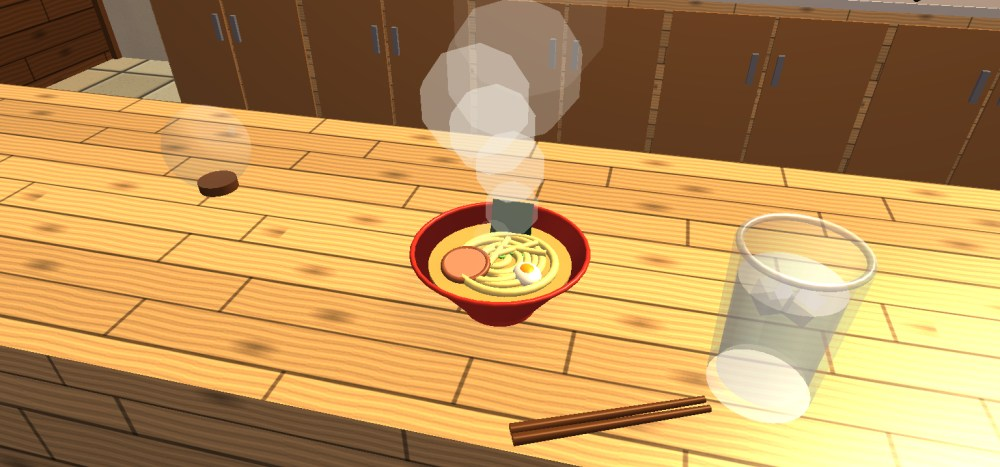
\includegraphics[width=\linewidth,trim=60 20 640 250,clip]{fig_bowlcam.jpg}\caption{Wood}\end{subfigure}\hfill
\begin{subfigure}{0.24\textwidth}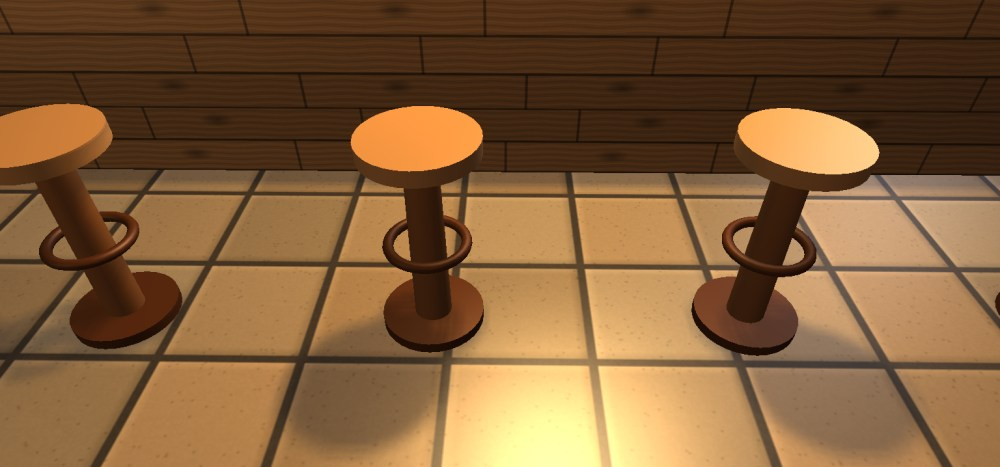
\includegraphics[width=\linewidth,trim=620 0 130 250,clip]{fig_stool_on.jpg}\caption{Floor tile}\end{subfigure}\hfill
\begin{subfigure}{0.24\textwidth}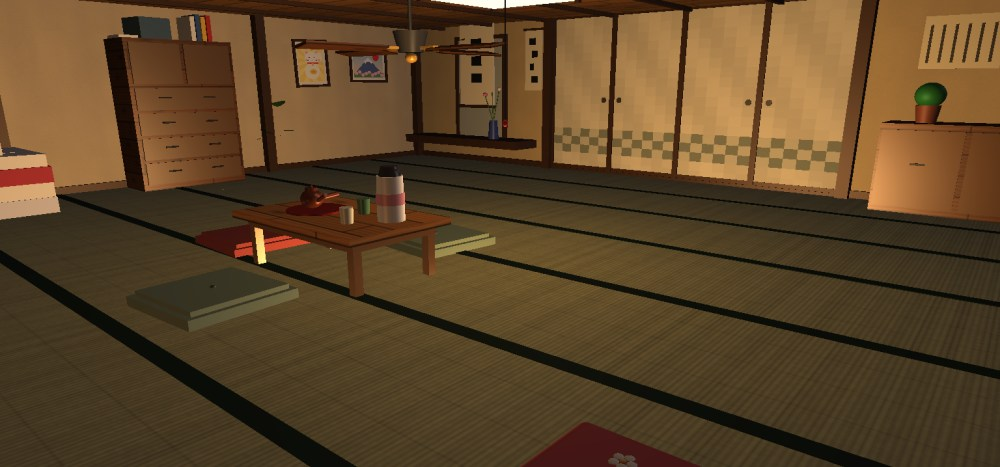
\includegraphics[width=\linewidth,trim=10 200 640 20,clip]{fig_up_orbit.jpg}\caption{Tatami}\end{subfigure}\hfill
\begin{subfigure}{0.24\textwidth}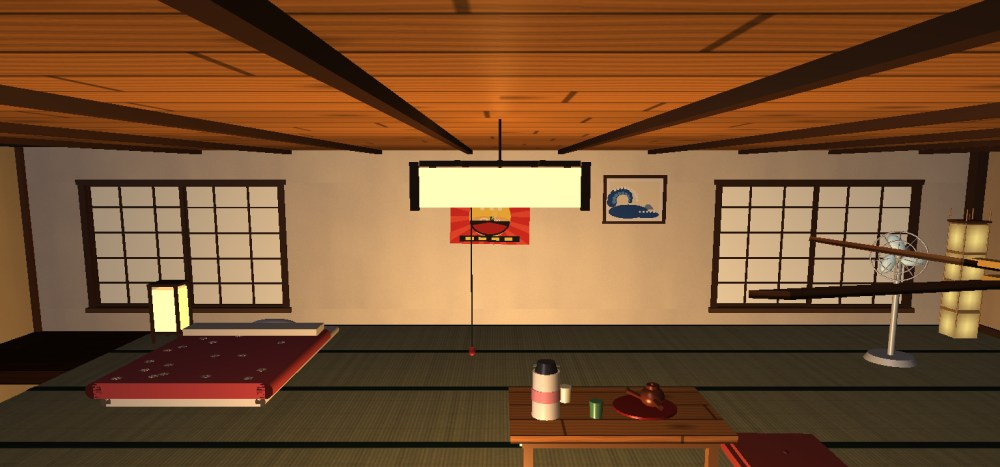
\includegraphics[width=\linewidth,trim=200 0 450 280,clip]{fig_up_windows.jpg}\caption{Ceiling boards}\end{subfigure}
\caption{Result: the procedural textures. Tatami uses a rounded reed profile $k=0.78+0.22\sin\pi f+\text{row tone}+\text{fibre}$.}\label{fig:tex}
\end{figure}

\subsection{Skybox, sun, moon, stars, clouds and day / night}\label{sec:sky}
\textbf{Theory.} A \emph{skybox} is drawn first with the depth test and depth write off and with the camera translation removed from the modelview matrix (only rotation kept), so it appears infinitely far and everything else is drawn over it. Glowing objects add light, so halos use \emph{additive blending}, $C=\alpha C_s+C_d$; ordinary transparency uses $C=\alpha C_s+(1-\alpha)C_d$. A \emph{billboard} is a quad rotated to always face the camera.\\
\textbf{Implementation.} \code{drawSky()} draws four layers (Table~\ref{tab:sky}); key \code{T} switches day and night, changing the sky colours, the sun/moon light colour (warm gold or cool blue), the lantern and window glow, the street lamps, the fog density ($0.012$ or $0.022$) and the shadows.
\begin{table}[htbp]
\centering\small
\begin{tabular}{@{}p{2.2cm}p{14.1cm}@{}}
\toprule
\textbf{Layer} & \textbf{Construction}\\
\midrule
Dome & 14 rings of 36 triangle strips, radius 150, elevation $-10^\circ$ to $90^\circ$; vertex colour $=\operatorname{mix}(\text{horizon},\text{zenith},t)$ with $t=(e/90^\circ)^{0.55}$. Day $(0.64,0.79,0.93)\to(0.17,0.40,0.80)$; night $(0.10,0.10,0.16)\to(0.015,0.02,0.07)$. By day the horizon equals the fog colour.\\
Sun & five camera-facing triangle-fan discs at direction $(45,7,-63)$: halos of radius 26, 13, 7 (alpha $0.12/0.22/0.35$ fading to 0 at the rim, additive), core radius 3, bloom radius 4; warm yellow to white\\
Moon & same position at night: cool halos (24, 11, 6), disc radius 2.8 and six darker craters (fans of radius 0.3--0.7, alpha $0.55\to0$)\\
Stars & 132 points (57 bright of 3 px, 75 dim of 1.5 px); brightness $0.7+0.3\sin(\omega_it+\varphi_i)$\\
Clouds & 12 clouds $\times$ 22 billboards, one 128$\times$128 RGBA noise sprite, flat base and domed top, sorted low to high, drifting with $a_0+vt$\\
\bottomrule
\end{tabular}
\caption{Layers of the sky.}\label{tab:sky}
\end{table}
\begin{Verbatim}
glDisable(GL_DEPTH_TEST);  glDepthMask(GL_FALSE);  glDisable(GL_FOG);
glGetFloatv(GL_MODELVIEW_MATRIX, mv);  mv[12] = mv[13] = mv[14] = 0;  glLoadMatrixf(mv);  // rotation only
drawGradientDome();  drawSunOrMoon();  if (night) drawStars();  drawCloudBillboards();
glDepthMask(GL_TRUE);  glEnable(GL_DEPTH_TEST);                                              // scene on top
\end{Verbatim}
\begin{figure}[htbp]
\centering
\begin{subfigure}{0.325\textwidth}\fig{1}{r_cyclist.jpg}\caption{Day: sun glow and sky}\end{subfigure}\hfill
\begin{subfigure}{0.325\textwidth}\fig{1}{r_moon.jpg}\caption{Night: cratered moon}\end{subfigure}\hfill
\begin{subfigure}{0.325\textwidth}\fig{1}{r_stars.jpg}\caption{Night: stars and clouds}\end{subfigure}
\caption{Result: sun, moon, stars and clouds.}\label{fig:sky}
\end{figure}

\subsection{Blending, transparency, emission and fog}
\textbf{Theory.} Fog mixes the colour with a fog colour by $f=e^{-(\rho z)^2}$ (exponential-squared): $C=fC_{surface}+(1-f)C_{fog}$. Transparent objects must be drawn after opaque ones, with depth \emph{writes} off, because the depth buffer cannot sort translucent surfaces.\\
\textbf{Implementation.} Glass, water, steam, clouds and soft shadows use alpha blending; halos, glows, light cones and fireflies use additive blending. All glass is drawn in a final transparent pass (\code{drawTransparentPass}). Steam is seven translucent spheres per bowl with phase $\varphi=(0.65t+\text{offset}+i/7)\bmod1$, radius $(0.09+0.32\varphi)$ and alpha $0.28\sin\pi\varphi$. Fog is applied in the Phong shader (and by \code{glFog} in the fixed path) with $\rho=0.012$ by day and $0.022$ at night.

\subsection{Shadows}\label{sec:shadow}
\textbf{Theory.} \emph{Planar projective shadow:} a point is flattened onto the plane $y=h$ along the light direction $\mathbf s$ (toward the light):
\begin{equation}
x'=x-\frac{s_x}{s_y}(y-h),\qquad y'=h,\qquad z'=z-\frac{s_z}{s_y}(y-h),
\end{equation}
a single $4\times4$ matrix; for a point light at $\mathbf l$, $x'=\dfrac{l_yx-l_xy}{l_y-y}$. \emph{Shadow mapping} (Williams~[5]) renders the scene from the light into a depth texture; a pixel with light-space depth $z_L$ is in shadow if $z_L>z_{map}+\epsilon$. \emph{Percentage-closer filtering}~[6] averages several comparisons, $s=\frac1N\sum_k[z_L\le z_{map,k}+\epsilon]$, for a soft edge.\\
\textbf{Implementation.} (1)~\emph{Sun shadows:} the whole outdoor scene is drawn a second time with the flattening matrix into the \textbf{stencil buffer} only (colour and depth writes off); then one soft dark layer is blended where the stencil is set, so overlapping shadows never darken twice. Depth testing is off for this pass (the plane is a few millimetres above the ground and would z-fight). (2)~\emph{Interior:} furniture is projected from the pendant and table lamps onto the tile floor with the point-light matrix and a stencil counter. (3)~\emph{Soft shadows (key \code{Y}):} the counter, stools, tables, chairs and bowls are drawn from the pendant light into a $512\times512$ depth texture (FOV $120^\circ$, \code{glPolygonOffset} against acne); in the fragment shader every pixel is moved to light space and compared $3\times3$ times, $1.5$ texels apart (each already a bilinear $2\times2$ hardware compare) and averaged (\code{pendantShadow()} above). The stencil pass of the sun shadow (\code{shadowLayer} in \code{scene.cpp}, shortened):
\begin{Verbatim}
glDisable(GL_DEPTH_TEST);  glEnable(GL_STENCIL_TEST);
glStencilFunc(GL_EQUAL, 0, 0xFF);               // exterior ground only (stencil 0)
glStencilOp(GL_KEEP, GL_KEEP, GL_INVERT);       // first fragment flips 0 -> 0xFF, later ones fail
glColorMask(0,0,0,0);  glDepthMask(GL_FALSE);   // write only the stencil
glPushMatrix();  multShadowMatrix(mode, lx, ly, lz, groundY);  drawExteriorBody();  glPopMatrix();
glColorMask(1,1,1,1);
glStencilFunc(GL_EQUAL, 0xFF, 0xFF);  glStencilOp(GL_KEEP, GL_KEEP, GL_ZERO);   // blend once, clear mask
glEnable(GL_BLEND);  glColor4f(0.01, 0.03, 0.01, alpha);  shadowRegion(sidewalk, groundY);   // dark layer
\end{Verbatim}
\begin{figure}[htbp]
\centering
\begin{subfigure}{0.325\textwidth}\fig{1}{fig_ext_day.jpg}\caption{Sun shadows (stencil)}\end{subfigure}\hfill
\begin{subfigure}{0.325\textwidth}\fig{1}{fig_sh_off.jpg}\caption{Projected only}\end{subfigure}\hfill
\begin{subfigure}{0.325\textwidth}\fig{1}{fig_sh_on.jpg}\caption{Shadow map + PCF}\end{subfigure}
\caption{Result: the three shadow methods.}
\end{figure}

\subsection{Glass refraction (screen space)}\label{sec:glass}
\textbf{Theory.} Snell's law $n_1\sin\theta_1=n_2\sin\theta_2$ bends a ray entering glass ($n=1.5$); the direction is $\mathbf t=\eta\mathbf d+(\eta c-\sqrt{1-\eta^2(1-c^2)})\mathbf n$ with $\eta=n_1/n_2$, $c=-\mathbf n\!\cdot\!\mathbf d$. The reflected share is Schlick's approximation~[7] $F=F_0+(1-F_0)(1-\cos\theta)^5$, $F_0=\big(\frac{n_1-n_2}{n_1+n_2}\big)^2\approx0.04$.\\
\textbf{Implementation.} The tumbler on the left table is drawn last. The screen behind it is copied into a texture; a GLSL shader offsets the texture lookup by the amount \code{refract(I, N, 1/1.5)} bends the view ray at the glass normal, and adds $F$ times the reflected room colour and a sharp lamp highlight ($n=140$). Only what is already on screen can be refracted, so this is an approximation (key \code{Z}).
\begin{figure}[htbp]
\centering
\begin{subfigure}{0.22\textwidth}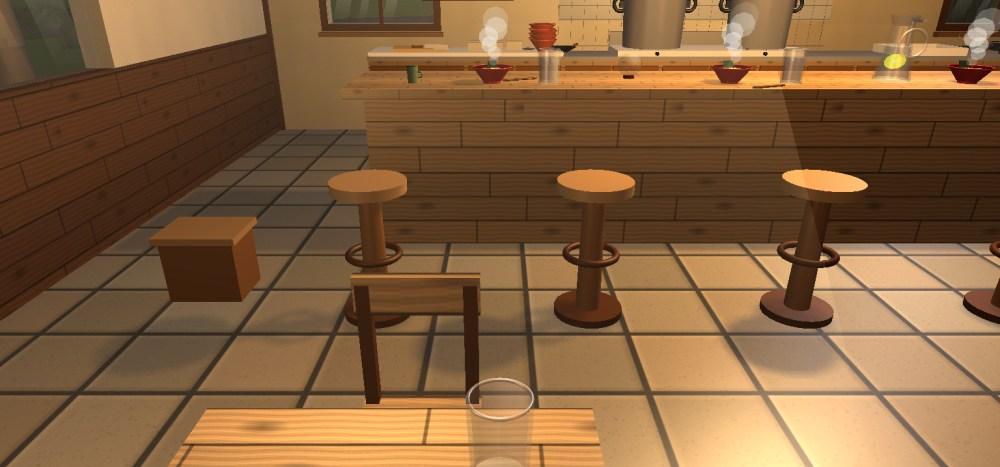
\includegraphics[width=\linewidth,trim=300 0 300 250,clip]{fig_refr_off.jpg}\caption{\code{Z} off}\end{subfigure}\hspace{0.03\textwidth}
\begin{subfigure}{0.22\textwidth}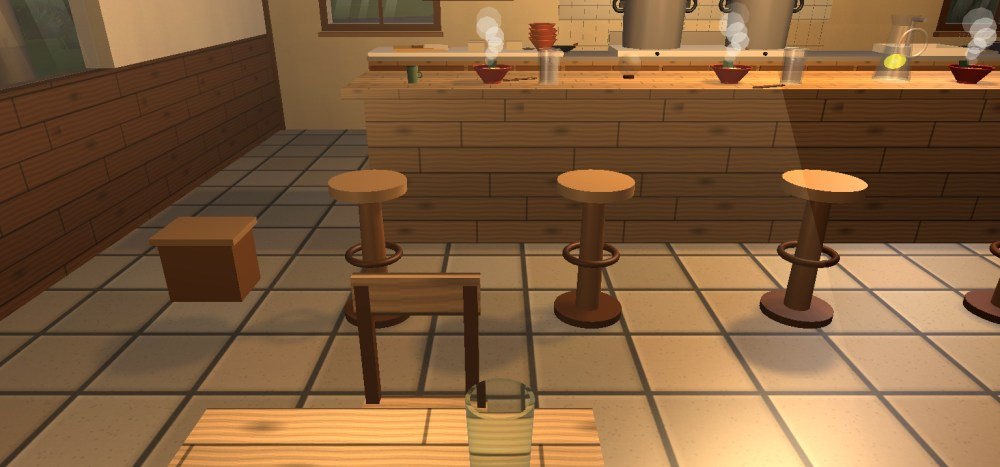
\includegraphics[width=\linewidth,trim=300 0 300 250,clip]{fig_refr_on.jpg}\caption{\code{Z} on}\end{subfigure}
\caption{Result: the tumbler without and with refraction.}
\end{figure}

\subsection{Ray tracing}\label{sec:rt}
\textbf{Theory.} Rasterisation asks for each triangle which pixels it covers; ray tracing asks for each pixel which object its ray hits. A ray is $\mathbf r(t)=\mathbf o+t\mathbf d$, $t>0$. At the nearest hit (point $\mathbf p$, normal $\mathbf n$) the colour is the local Blinn--Phong colour plus recursive rays (Whitted~[4]): a \emph{reflection} ray $\mathbf r=\mathbf d-2(\mathbf d\!\cdot\!\mathbf n)\mathbf n$ and, for glass, a \emph{refraction} ray $\mathbf t$ (Snell's law above; if $1-\eta^2(1-c^2)<0$ the ray is totally internally reflected). They are weighted by the Fresnel term, $C=(1-F)C_{local\text{ or }refr}+F\,C_{refl}$. Intersections: for a \textbf{sphere} $|\mathbf p-\mathbf c|^2=R^2$ substituting the ray gives $|\mathbf d|^2t^2+2\,\mathbf d\!\cdot\!(\mathbf o-\mathbf c)\,t+|\mathbf o-\mathbf c|^2-R^2=0$ (discriminant $<0$: miss); for a \textbf{plane/disk} $t=\frac{(\mathbf q-\mathbf o)\cdot\mathbf n}{\mathbf d\cdot\mathbf n}$ then a radius test; for an \textbf{axis-aligned box} the slab method, $t_{1,2}=(b_{min,max}-o)/d$ per axis, hit if $\max t_{near}\le\min t_{far}$; for a \textbf{cone / frustum} a quadratic in $t$ whose root must lie in the height range. A \textbf{bounding volume hierarchy} (BVH) wraps groups of shapes in boxes so a ray that misses a box skips everything inside it: the cost per ray falls from $O(n)$ to about $O(\log n)$.\\
\textbf{Implementation} (\code{rtcore.cpp}, \code{rtscene.cpp}, \code{rtpass.cpp}; key \code{R}).
\begin{itemize}
\item \textbf{What is traced:} the 2 steel stock pots, the 4 ramen bowls, the glass ball on the counter and the mirror upstairs (8 objects). The rest of the frame stays OpenGL.
\item \textbf{Scene:} \code{rtBuildShopScene} rebuilds the shop for the rays from the same positions and sizes as the OpenGL models (boxes, truncated cones, disks, spheres), with CPU copies of the textures and the live OpenGL lights; lamps are emissive shapes so they appear in reflections. The BVH uses a median split on the longest axis with at most 2 shapes per leaf; large floors and walls are tested directly.
\item \textbf{Shading:} metal, glaze, soup and the mirror add a reflection ray $\times F$ (up to \code{maxDepth}=3); the glass ball applies Snell's law at every surface, with total internal reflection.
\item \textbf{Speed:} only the screen rectangle of each traced object is processed, rows are shared by up to 8 threads, and a ray budget keeps the pass near 25\,ms by tracing one ray per $2\times2$ (or larger) block when a big area is on screen; measured about 13\,ms in Release (7\,000 eye rays), 80\,ms in Debug.
\item \textbf{Compositing:} a shader draws the result over the OpenGL frame only where the depth buffer shows the same surface, so nearer objects still hide a pot.
\end{itemize}
The recursion of the tracer (\code{radiance} and \code{glassRadiance} in \code{rtcore.cpp}, simplified):
\begin{Verbatim}
radiance(o, d, depth):
    hit = bvhIntersect(o, d)                       // nearest shape; big floors/walls tested directly
    if no hit: return skyColour
    N = normal facing the ray;  V = -d
    EMISSIVE: return emission                      // lamps: they show up in reflections
    DIFFUSE : return blinnPhong(hit, N, V)         // all lights, no shadow rays
    GLASS   : return glassRadiance(hit, d, depth)
    METAL / GLAZE / LIQUID / MIRROR:
        F = schlick(f0, dot(N,V));  local = blinnPhong(hit, N, V)
        if depth >= maxDepth: return local
        return local*(1-F) + radiance(p+N*eps, reflect(d,N), depth+1) * F

glassRadiance(hit, d, depth):                      // follows the ray through up to 10 surfaces
    repeat:  entering = dot(d,n) < 0;  eta = entering ? 1/ior : ior
             t = refract(d, n, eta)                // fails => total internal reflection
             F = tir ? 1 : R0 + (1-R0)*(1-cos)^5
             if first surface: colour += radiance(p, reflect(d,n), depth+1) * F
             if tir: d = reflect(d,n)  else: { throughput *= (1-F);  d = t }
             next = next surface of the same glass object, else the whole scene
             if next is not glass: return colour + throughput * radiance(p, d, depth+1)
\end{Verbatim}
\begin{figure}[htbp]
\centering
\begin{subfigure}{0.325\textwidth}\fig{1}{fig_rtc_off.jpg}\caption{OpenGL only}\end{subfigure}\hfill
\begin{subfigure}{0.325\textwidth}\fig{1}{r_bowlrt.jpg}\caption{Ray tracing: glaze, ball}\end{subfigure}\hfill
\begin{subfigure}{0.325\textwidth}\fig{1}{r_mirror.jpg}\caption{Mirror upstairs}\end{subfigure}
\caption{Result: ray tracing (key \code{R}). The glaze mirrors the lamps, the glass ball refracts the counter, the mirror reflects the room.}\label{fig:rt}
\end{figure}

\subsection{Animation and the characters}\label{sec:anim}
\textbf{Theory.} Every motion is a function of one clock $t$ (\code{animTime}, advanced by a 16\,ms timer; \code{Space} pauses). A wheel that has rolled a distance $d$ has turned $\theta=d/r$. A joint chain is \emph{forward kinematics} (a stack of rotations); \emph{inverse kinematics} finds the joint from the target: for a two-bone limb with hip $\mathbf h$, foot $\mathbf f$, bone lengths $L_1,L_2$ and $d=|\mathbf f-\mathbf h|$,
\begin{equation}
a=\frac{L_1^2-L_2^2+d^2}{2d},\qquad h=\sqrt{L_1^2-a^2},\qquad \mathbf k=\mathbf h+a\,\hat{\mathbf u}+h\,\hat{\mathbf u}^{\perp}.
\end{equation}
Smooth easing uses $3k^2-2k^3$. A pendulum with wind obeys $\ddot\theta=-\frac gL\sin\theta-c\dot\theta+kw(t)$, integrated by semi-implicit Euler steps ($\dot\theta\leftarrow\dot\theta+\ddot\theta\Delta t$, then $\theta\leftarrow\theta+\dot\theta\Delta t$).\\
\textbf{Implementation} (\code{scene.cpp}). A helper \code{limb(a,b,r)} draws a cylinder between two points.
\begin{itemize}
\item \textbf{Cyclist} (\code{drawBicycle}): rides $x=-16\ldots16$ at 7 units/s, scale $1.4$. Wheel angle $-d/(rS)$; two cranks of length $0.17$ turn at $0.55\,d/(rS)$ and the legs ($L_1=L_2=0.47$) reach the pedals by the IK above; the frame is seven red tubes; a headlight and an additive road beam at night; shadow on the cobblestones.
\begin{Verbatim}
dist  = fmod(animTime*7, 32);   x = -16 + dist;                  // 7 units/s, loops every 32 units
wheelDeg = -(dist / (R*SC)) * 57.29578;                          // rolling without slipping
crank    = -(dist / (R*SC)) * 0.55;                              // pedals turn slower than wheels
for each pedal p:  P[p] = bottomBracket + 0.17*(cos(a), sin(a));  a = crank + p*PI
    knee = kneeFor(hip, P[p], 0.47, 0.47);                       // two-bone IK (law of cosines)
    limb(hip, knee, 0.055);  limb(knee, P[p], 0.045);            // thigh, shin
\end{Verbatim}
\item \textbf{Walking person} (\code{drawWalkingPerson}): $1.8$ units/s, joint hierarchy hip $\to$ thigh $0.46$ $\to$ knee $\to$ shin $0.44$; with stride phase $\varphi=2\pi\cdot1.8t/1.4$: thigh $\pm28^\circ\sin\varphi$, knee bend $35^\circ\max(0,\sin(\varphi+\varphi_0))$, arms swing $-0.8\times$ the leg angle, body bob $0.035|\cos\varphi|$.
\item \textbf{Cat} (\code{drawWalkingCat}): walks at 3 units/s; every \emph{third lap} a time-driven state machine stops it at $x=-1.2$, turns it to the street (smoothstep over $0.5$ s), sits it down and washes its face for 7 s (paw lick $\sin9t_w$, wipe $0.5+0.5\sin2.2t_w$, head tilt $-14^\circ+10^\circ\cdot$wipe, then looks around $25^\circ\sin0.8t$); walking uses diagonal leg pairs with swing $0.06\sin(\varphi+\varphi_i)$, lift $0.025\max(0,\cos(\varphi+\varphi_i))$, tail swaying.
\item \textbf{Wind chime} (\code{drawFurin}): bell ($L_1=0.12$) and paper strip ($L_2=0.20$) are two pendulums with wind gains $k_1=3$, $k_2=22$, 8 sub-steps per frame; when $|\theta_2-\theta_1|>0.42$ rad the clapper strikes, rebounds with $-0.45$ of the relative speed and a glint flashes. \textbf{Banner:} grid wave of Section~\ref{sec:model}. \textbf{Fans:} blades $160^\circ$/s and $900^\circ$/s.
\end{itemize}
\begin{figure}[htbp]
\centering
\begin{subfigure}{0.52\textwidth}\fig{1}{r_cyclist.jpg}\caption{Cyclist with shadow}\end{subfigure}\hfill
\begin{subfigure}{0.40\textwidth}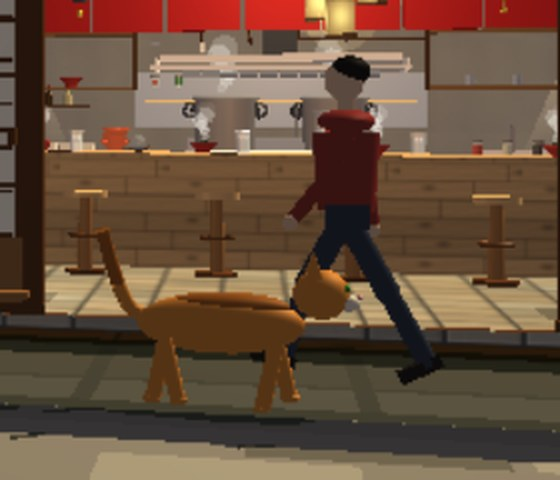
\includegraphics[width=\linewidth]{r_pc.jpg}\caption{Person and cat}\end{subfigure}
\caption{Result: the animated characters on the cobblestone street.}\label{fig:cyc}
\end{figure}

\subsection{The environment and the buildings}\label{sec:env}
\begin{table}[htbp]
\centering\footnotesize
\begin{tabular}{@{}p{3.3cm}cp{11.2cm}@{}}
\toprule
\textbf{Object (function)} & \textbf{Count} & \textbf{How it is made}\\
\midrule
Cherry tree (\code{drawCherryBlossomTree}) & 7 & 3-level recursion, pink blossom clusters, falling petals (14) and petal carpet (110)\\
Maple (\code{drawMapleTree}) & 6 & 4-level finer branching, red-orange notched leaves\\
Broadleaf (\code{drawTree}) & 6 & 3 levels, leaf pads on tips and mid-branch, flared trunk with 5 roots\\
Pine (\code{drawJapanesePineTree}) & 5 & trunk 3.3 tall, stacked jagged triangle-fan skirts, swaying crown\\
Bamboo (\code{drawBambooGrove}) & 2 & culms $4.6$--$6.6$ tall, 9--11 nodes, lean, age-dependent green--yellow\\
Jungle, flowers & 8, 9 & dome bushes and fern fronds; 40 flowers per garden on a golden-angle spiral, 7 colours\\
Lake (\code{drawLake}), bridge, ducks & 1, 1, 2 & disc radius 8 with scrolling water texture and rippling rim, 12 rocks, 4 lily pads; arched bridge of 34 planks ($y=0.6\cos(\pi z/17)$); ducks on circles of radius $3.5$ with a wake\\
Fireflies & 129 & 8 groups; orbit, pulse $0.5+0.5\sin(\omega t+\varphi)$ and on/off phase; additive\\
Street lamps, stone lanterns & 12, 4 & pole 3.3, arm, shade; emissive bulb, additive light cone and ground pool at night\\
Houses (\code{drawJapaneseHouse}, \code{...2}) & 10 & type 1: $4\times3.5$, veranda, 4 red lanterns; type 2: $6\times3.5$ on raised floor, 4 sliding shoji panels, side porch; textured walls and roof\\
Shop (\code{drawShopBuilding}, \code{drawRoof}) & 1 & $10\times8$ floor, plaster walls with openings, gable roof $11.4\times2.2\times9.4$, awning with 37 blue cones, sign, shoji windows that glow only when an interior lamp is on, 2 swaying lanterns, doors opened by click\\
Dining room, kitchen & -- & counter, 6 stools, 2 tables, 4 chairs, 4 bowls with steam, 2 stock pots, stove, hood, fridge, sink, pendant lamps, lanterns, noren, clock, glassware\\
Upstairs room & -- & staggered tatami, fusuma and shoji doors, futon, tea table with teapot, tansu chest, radio, fans, mirror, 6 pictures drawn from 2D shapes (clipped by Sutherland--Hodgman~[8])\\
\bottomrule
\end{tabular}
\caption{The objects of the scene and how they are made.}
\end{table}
\begin{figure}[htbp]
\centering
\begin{subfigure}{0.325\textwidth}\fig{1}{r_village.jpg}\caption{Shop, cherry and maple trees}\end{subfigure}\hfill
\begin{subfigure}{0.325\textwidth}\fig{1}{r_house1.jpg}\caption{Neighbouring house (type 1)}\end{subfigure}\hfill
\begin{subfigure}{0.325\textwidth}\fig{1}{r_pond.jpg}\caption{Lake, bridge, ducks}\end{subfigure}\\[2pt]
\begin{subfigure}{0.325\textwidth}\fig{1}{r_dining1.jpg}\caption{Dining room and kitchen}\end{subfigure}\hfill
\begin{subfigure}{0.325\textwidth}\fig{1}{r_bowl.jpg}\caption{Ramen bowl with steam}\end{subfigure}\hfill
\begin{subfigure}{0.325\textwidth}\fig{1}{r_upper1.jpg}\caption{Upstairs tatami room}\end{subfigure}
\caption{Result: the village and the inside of the shop.}
\end{figure}

\subsection{Interaction and the cooking game}\label{sec:game}
Keyboard and mouse events arrive through GLUT callbacks and change global state that the next frame reads: \code{C} camera, \code{T} day/night, \code{1--7} lamps, \code{G} shading, \code{Y} soft shadows, \code{Z} refraction, \code{R} ray tracing, \code{H} roof, \code{F} fog, \code{X} steam, \code{Tab} select an object to move (\code{I J K L U N}), rotate (\code{[ ]}) and scale (\code{, .}). The game (\code{game.cpp}, \code{Enter}) is a state machine MENU $\to$ TAKING\_ORDER $\to$ COOKING $\to$ SERVING $\to$ RESULT: a customer orders, the player boils noodles (raw $<3$ s, perfect 6--9 s, ruined $>12$ s), adds broth and toppings and serves. Score $Q=0.5\,\text{accuracy}+0.35\,\text{cook}+0.15\,\text{time}$, stars $=\operatorname{round}(5Q)$, up to four levels; the HUD uses the orthographic projection.
\begin{figure}[htbp]
\centering
\begin{subfigure}{0.325\textwidth}\fig{1}{fig_game_menu.jpg}\caption{Title}\end{subfigure}\hfill
\begin{subfigure}{0.325\textwidth}\fig{1}{fig_game_order.jpg}\caption{Order board}\end{subfigure}\hfill
\begin{subfigure}{0.325\textwidth}\fig{1}{fig_game_cust.jpg}\caption{Customer}\end{subfigure}
\caption{Result: the game screens.}\label{fig:game}
\end{figure}

% ===================== 6 RESULTS / DISCUSSION =====================
\section{Results, Problems and Limitations}
The scene runs in real time with all effects on (Figure~\ref{fig:res}); ray tracing adds about 13\,ms per frame in a Release build. Scene statistics: 8 lights (7 switchable fixtures), 13 textures, 7 cameras, 10 houses, 12 street lamps, 24 trees, 132 stars, 12 clouds, 8 ray-traced objects, 3 animated characters and a $512^2$ shadow map.
\begin{figure}[htbp]
\centering
\begin{subfigure}{0.49\textwidth}\fig{1}{fig_ext_day2.jpg}\caption{Day}\end{subfigure}\hfill
\begin{subfigure}{0.49\textwidth}\fig{1}{fig_ext_night.jpg}\caption{Night}\end{subfigure}
\caption{The finished scene by day and at night.}\label{fig:res}
\end{figure}
\textbf{Problems and solutions.}
\begin{itemize}
\item \emph{Only 8 lights:} outdoor lights are re-assigned to interior fixtures while the inside is drawn, and a shader mask keeps outside lights from lighting the interior through the walls.
\item \emph{Lights off but the room still lit:} a global ambient and glowing materials caused it; the global ambient is now zero and glowing surfaces fade with their lamp.
\item \emph{Broken, streaky shadows:} the shadow plane z-fought with the ground and leaf cards left gaps in the stencil; depth testing is off in that pass and trees use full leaf geometry near the shop.
\item \emph{Blocky ray-traced objects up close:} the ray budget keeps the cost bounded, so one ray covers several pixels; the drinking glasses and jug were therefore moved back to OpenGL.
\end{itemize}
\textbf{Limitations.} No flat shading; refraction of the tumbler is screen-space; ray tracing covers only 8 interior objects and has no shadow rays; night shadows outdoors are simple fixed shapes; no sound. \textbf{Future work:} cube-map shadows for every lamp, a GPU ray tracer, customers that walk into the shop by themselves.

\section{Conclusion}
The Ramen Shop implements the proposed features (translation, rotation, scaling, perspective camera, hierarchical modelling, ambient, diffuse and specular lighting, Gouraud and Phong shading, skybox, textures; the orthographic view is used for the HUD, and flat shading was not implemented) and adds shadows, glass refraction, ray tracing with a BVH, animated characters, a procedural environment with my own grass and cobblestone textures, and a cooking game, all in one Visual Studio project with no external assets.

\begin{thebibliography}{10}\footnotesize
\bibitem{phong} B.~T.~Phong, ``Illumination for computer generated pictures,'' \emph{Communications of the ACM} 18(6), 1975.
\bibitem{blinn} J.~F.~Blinn, ``Models of light reflection for computer synthesized pictures,'' \emph{SIGGRAPH}, 1977.
\bibitem{gouraud} H.~Gouraud, ``Continuous shading of curved surfaces,'' \emph{IEEE Trans.\ Computers} C-20(6), 1971.
\bibitem{whitted} T.~Whitted, ``An improved illumination model for shaded display,'' \emph{Communications of the ACM} 23(6), 1980.
\bibitem{williams} L.~Williams, ``Casting curved shadows on curved surfaces,'' \emph{SIGGRAPH}, 1978.
\bibitem{reeves} W.~Reeves, D.~Salesin, R.~Cook, ``Rendering antialiased shadows with depth maps,'' \emph{SIGGRAPH}, 1987.
\bibitem{schlick} C.~Schlick, ``An inexpensive BRDF model for physically-based rendering,'' \emph{Eurographics}, 1994.
\bibitem{sh} I.~Sutherland, G.~Hodgman, ``Reentrant polygon clipping,'' \emph{Communications of the ACM} 17(1), 1974.
\bibitem{redbook} D.~Shreiner et al., \emph{OpenGL Programming Guide} (the ``Red Book''), Addison-Wesley; Khronos, \emph{OpenGL and GLSL 1.20 specifications}.
\bibitem{noise} D.~Ebert et al., \emph{Texturing and Modeling: A Procedural Approach}, Morgan Kaufmann (value noise, fractal Brownian motion).
\end{thebibliography}

\end{document}
